\chapter{Conformal Mapping, Laplace's Equation, and Open-String Scattering}

Let us begin exactly where Leonard Susskind begins. Conformal mappings are not introduced here as a technical convenience of string theory. They are interesting in their own right, they are widely useful in mathematical physics, and the most direct example for this lecture is two-dimensional electrostatics. These notes follow that lecture order, with the blackboard record preserved through the curation of LazyingArt LLC and Video2Book, so that the mathematics can unfold with the same motivation and rhythm.

\section{Electrostatics As The First Model For Conformal Mapping}

Susskind starts by being careful about what he means by electrostatics in two dimensions. He does not mean charges constrained to move in a plane while still interacting with the ordinary three-dimensional Coulomb law. He means a literal two-dimensional world, one in which electric flux lines are forced to lie in the plane. In such a world the Coulomb force is not \(1/r^2\), but
\begin{equation}
F(r)\propto \frac{1}{r},
\end{equation}
and therefore the potential energy is logarithmic,
\begin{equation}
V(r)\propto \log r.
\end{equation}
The mathematics is already different before conformal mapping enters.

The next move is characteristic of the lecture. Rather than working directly with the electric field, we pass to a simpler object, the scalar potential \(\phi\). Keeping the lecture's sign convention,
\begin{align}
\mathbf E &= \nabla \phi, \\
\nabla\cdot \mathbf E &= \rho.
\end{align}
Combining these gives the Poisson equation
\begin{equation}
\nabla^2\phi=\rho.
\end{equation}
Now unpack the Laplacian in a literal two-dimensional world with coordinates \(x\) and \(y\):
\begin{equation}
\nabla^2\phi
=
\frac{\partial^2\phi}{\partial x^2}
+
\frac{\partial^2\phi}{\partial y^2}.
\end{equation}
Where there is charge density this equals \(\rho\); where there is no charge density it reduces to Laplace's equation,
\begin{equation}
\frac{\partial^2\phi}{\partial x^2}
+
\frac{\partial^2\phi}{\partial y^2}
=0.
\end{equation}

\begin{figure}[h]
\centering

\includegraphics[width=0.62\textwidth]{lecture_08_figure_02.png}
\caption{Electrostatic equations and the two-dimensional Laplacian.}
\end{figure}

This is the equation that matters. The point of the opening is not merely to remind us of electrostatics, but to put a definite invariant equation on the board. Conformal transformations preserve angles, and in two dimensions they preserve the form of Laplace's equation. That is why one can take a solution on one domain, map the domain, and carry the solution with it to a new geometry. Susskind mentions cartography and fluid flow for the same reason: the mathematics is broader than string theory, even though string theory is where we are headed.

\subsection{Question \& Answer}

\paragraph{Question.} Why are these not wave equations?

\paragraph{Answer.} Because the equation on the board is purely spatial and has the elliptic sign structure
\[
\partial_x^2\phi+\partial_y^2\phi=0.
\]
There is no time derivative, and the two spatial second derivatives come with the same sign. If we wanted waves, we would have to add time dependence. Electrostatics is static precisely because nothing is moving.

A student then asks about curl in two dimensions, and Susskind uses the question as a bridge rather than a digression. If
\[
\mathbf E=(E_x,E_y),
\]
then in two dimensions the curl has only one component,
\begin{equation}
\operatorname{curl}_{2d}\mathbf E
=
\frac{\partial E_x}{\partial y}
-
\frac{\partial E_y}{\partial x}.
\end{equation}
One may think of it as the component perpendicular to the board if one likes, but the real point is simpler: in two dimensions the curl becomes a one-component object. We will meet this again once \(u\) and \(v\) begin to behave like the components of a vector field.

\section{Complex Coordinates And The Problem Of A Unique Derivative}

Having motivated conformal invariance through Laplace's equation, the lecture shifts to the right language for planar mappings. Write the original plane as
\begin{equation}
z=x+iy,
\end{equation}
and the image plane as
\begin{equation}
w=u+iv.
\end{equation}
A mapping of the plane to itself is then a complex function \(w(z)\), or equally well a coordinate transformation from \((x,y)\) to \((u,v)\). The lecture assumes the mapping is one-to-one, so every point on the \(z\)-plane determines a unique point on the \(w\)-plane, and vice versa. In that sense we are still doing coordinate transformations, only now in complex notation.

Susskind deliberately concentrates on differential rather than integral calculus. Suppose we move from a point \(z\) to a nearby point \(z+\Delta z\). The image point moves from \(w\) to \(w+\Delta w\). The obvious candidate for the derivative is
\begin{equation}
\frac{dw}{dz}
=
\lim_{\Delta z\to 0}\frac{\Delta w}{\Delta z}.
\end{equation}
The problem is that, unlike the real line, the complex plane allows infinitely many directions of approach. It is not enough that the function be continuous or even smooth in an ordinary sense. The ratio \(\Delta w/\Delta z\) might depend on how we come into the point.

\subsection{Question \& Answer}

\paragraph{Question.} What condition makes \(dw/dz\) well defined in the complex plane?

\paragraph{Answer.} The limit must be independent of direction. Susskind derives the condition by comparing approach along the \(x\)-axis with approach along the \(y\)-axis. If those agree, one gets the crucial equations; and in fact that condition turns out to be sufficient as well.

Along the \(x\)-axis we keep \(y\) fixed, so \(dy=0\). Then
\begin{equation}
\frac{dw}{dz}
=
\frac{\partial u}{\partial x}
+
i\frac{\partial v}{\partial x}.
\end{equation}
Along the \(y\)-axis we keep \(x\) fixed, so \(dx=0\). Then
\begin{equation}
\frac{dw}{dz}
=
\frac{1}{i}\frac{\partial u}{\partial y}
+
\frac{\partial v}{\partial y}
=
\frac{\partial v}{\partial y}
-
i\frac{\partial u}{\partial y}.
\end{equation}
If these are to represent the same derivative, their real parts and imaginary parts must match.

\section{Cauchy-Riemann Equations And Harmonic Functions}

Matching the two directional derivatives gives the Cauchy-Riemann equations:
\begin{align}
\frac{\partial u}{\partial x} &= \frac{\partial v}{\partial y}, \\
\frac{\partial u}{\partial y} &= -\,\frac{\partial v}{\partial x}.
\end{align}
This is the condition for the derivative \(dw/dz\) to exist in a unique, meaningful way. When the condition holds, the function is called analytic. If it holds everywhere, the lecture uses the standard name entire.

The lecture does not leave these equations as mere formal conditions. It immediately asks what they imply. Since they couple \(u\) and \(v\), can we uncouple them and write separate equations for each? Yes. Differentiate the first equation with respect to \(x\):
\begin{equation}
\frac{\partial^2 u}{\partial x^2}
=
\frac{\partial^2 v}{\partial x\,\partial y}.
\end{equation}
Differentiate the second with respect to \(y\):
\begin{equation}
\frac{\partial^2 u}{\partial y^2}
=
-\,\frac{\partial^2 v}{\partial x\,\partial y}.
\end{equation}
Add them and the mixed partial derivatives cancel:
\begin{equation}
\frac{\partial^2 u}{\partial x^2}
+
\frac{\partial^2 u}{\partial y^2}
=0.
\end{equation}
Exactly the same maneuver, with \(x\) and \(y\) interchanged in the right places, gives
\begin{equation}
\frac{\partial^2 v}{\partial x^2}
+
\frac{\partial^2 v}{\partial y^2}
=0.
\end{equation}

So an analytic function \(w=u+iv\) contains two real harmonic functions. This is the point of return to the opening electrostatics discussion. Complex differentiability has led us straight back to Laplace's equation.

There is also the brief curl-divergence interpretation prompted by a student question. If we regard \((u,-v)\) as the components of a two-dimensional vector field, then the Cauchy-Riemann equations read
\begin{align}
\frac{\partial u}{\partial x}
-
\frac{\partial v}{\partial y}
&=0, \\
\frac{\partial u}{\partial y}
+
\frac{\partial v}{\partial x}
&=0.
\end{align}
The first says the divergence vanishes; the second says the curl vanishes. That is why these equations look so familiar from the electrostatics side of the story.

The lecture also makes an important one-way caution. Every analytic function gives two harmonic functions, but not every pair of harmonic functions comes from an analytic function. The Cauchy-Riemann equations are what link the pair together.

\section{Why Analytic Functions Are Conformal}

Now comes the advertised payoff. Susskind says this quite plainly: that was the whole point. We want to show that analytic mappings are not merely examples of conformal mappings. They are the same thing.

The argument is local and geometric. First recall a simple fact about complex numbers. A small complex number can be written in polar form as
\begin{equation}
\delta z=\rho e^{i\theta},
\qquad
\Delta z=\rho' e^{i\theta'}.
\end{equation}
Then
\begin{equation}
\frac{\delta z}{\Delta z}
=
\frac{\rho}{\rho'}e^{i(\theta-\theta')}.
\end{equation}
The magnitude is not the issue. The phase is. The phase of a ratio is the difference of the phases, and that difference is exactly the angle between the two displacements.

Now return to the \(z\)-plane and the \(w\)-plane. At a point in the \(z\)-plane take two tiny intervals, \(\delta z\) and \(\Delta z\), meeting at that point. Under the mapping they go to \(\delta w\) and \(\Delta w\). If \(w(z)\) is analytic, the derivative is well defined and independent of direction, so
\begin{equation}
\frac{\delta w}{\delta z}
=
\frac{\Delta w}{\Delta z}.
\end{equation}
Rearranging,
\begin{equation}
\frac{\Delta z}{\delta z}
=
\frac{\Delta w}{\delta w}.
\end{equation}
But now the phase of the left-hand side is the angle between the two intervals in the \(z\)-plane, while the phase of the right-hand side is the angle between their images in the \(w\)-plane. Therefore those angles are equal. That is the conformal property.

\begin{figure}[h]
\centering
\begin{tikzpicture}[scale=1.0]
\draw[->] (-1.4,0) -- (1.6,0);
\draw[->] (0,-1.2) -- (0,1.6);
\node at (0,-1.5) {$z$-plane};
\fill (0,0) circle (0.04);
\draw[->] (0,0) -- (1.15,0.42);
\draw[->] (0,0) -- (0.48,1.12);
\node at (1.18,0.65) {$\delta z$};
\node at (0.72,1.28) {$\Delta z$};
\draw (0.48,0.17) arc (20:67:0.50);

\begin{scope}[xshift=5.2cm]
\draw[->] (-1.4,0) -- (1.6,0);
\draw[->] (0,-1.2) -- (0,1.6);
\node at (0,-1.5) {$w$-plane};
\fill (0,0) circle (0.04);
\draw[->] (0,0) -- (1.18,0.50);
\draw[->] (0,0) -- (0.54,1.18);
\node at (1.22,0.74) {$\delta w$};
\node at (0.78,1.34) {$\Delta w$};
\draw (0.50,0.21) arc (23:66:0.54);
\end{scope}
\end{tikzpicture}
\caption{Two infinitesimal intervals in the \(z\)-plane and their images in the \(w\)-plane. Analyticity preserves the angle between them.}
\end{figure}

\subsection{Question \& Answer}

\paragraph{Question.} Why does analyticity imply angle preservation?

\paragraph{Answer.} Because analyticity makes the derivative the same in every infinitesimal direction through the point. Once two intervals are compared by taking a ratio, the common derivative cancels. What remains is a ratio of complex intervals, and the phase of that ratio is the angle between them. Equal ratios therefore mean equal angles.

So the local statement is complete: analytic maps preserve angles, and that is why they are the coordinate transformations under which the two-dimensional equations of motion keep their form. This is exactly why they matter in string theory.

\section{Examples And Global Maps: \(z^2\), \(e^z\), \(\log z\), And The Disk}

Only after the proof does the lecture turn to examples. The order matters. These are not a detached catalogue of complex functions; they are meant to train our eye.

\paragraph{A first easy example: \(W=z^2\).} On the board the order is simple and clean:
\begin{align}
W &= z^2, \\
(x+iy)^2 &= x^2-y^2+2ixy=u+iv, \\
u &= x^2-y^2, \\
v &= 2xy.
\end{align}

\begin{figure}[h]
\centering

\includegraphics[width=0.72\textwidth]{lecture_08_figure_03.png}
\caption{The map \(W=z^2\) and the identification of \(u\) and \(v\).}
\end{figure}

Now check the harmonicity directly. For \(u=x^2-y^2\),
\begin{equation}
\frac{\partial^2 u}{\partial x^2}=2,
\qquad
\frac{\partial^2 u}{\partial y^2}=-2,
\end{equation}
so
\begin{equation}
\frac{\partial^2 u}{\partial x^2}
+
\frac{\partial^2 u}{\partial y^2}
=0.
\end{equation}
For \(v=2xy\),
\begin{equation}
\frac{\partial^2 v}{\partial x^2}=0,
\qquad
\frac{\partial^2 v}{\partial y^2}=0,
\end{equation}
and therefore \(v\) is harmonic as well. This is exactly the kind of example the lecture wants: algebra on the complex side, Laplace's equation on the real side.

\paragraph{A deliberate failure: \(w=\bar z\).} To see what non-analyticity looks like, take
\begin{equation}
w=\bar z=x-iy.
\end{equation}
Then
\begin{equation}
u=x,
\qquad
v=-y.
\end{equation}
But now
\begin{equation}
\frac{\partial u}{\partial x}=1,
\qquad
\frac{\partial v}{\partial y}=-1,
\end{equation}
so the first Cauchy-Riemann equation already fails. The culprit is the complex conjugate. Analytic functions are built from \(z\), not from \(\bar z\).

\paragraph{A richer analytic example: \(w=e^z\).} Write
\begin{equation}
w=e^z=e^{x+iy}=e^x(\cos y+i\sin y),
\end{equation}
so that
\begin{equation}
u=e^x\cos y,
\qquad
v=e^x\sin y.
\end{equation}
Then
\begin{align}
\frac{\partial u}{\partial x}
&=
e^x\cos y
=
\frac{\partial v}{\partial y},
\\
\frac{\partial u}{\partial y}
&=
-\,e^x\sin y
=
-\,\frac{\partial v}{\partial x}.
\end{align}
So \(e^z\) is analytic, exactly as expected.

At this point the lecture notes that the logarithm is the inverse function, and asks why the inverse of an analytic map is again analytic where it exists. The answer comes from the same conformal logic: if angles are preserved one way, they are preserved the other way as well. With that in mind, we pass naturally to
\begin{equation}
w=\log z.
\end{equation}

Write
\begin{equation}
z=re^{i\theta}.
\end{equation}
Then
\begin{equation}
w=\log z=\log r+i\theta.
\end{equation}
Now restrict attention to the right half-plane. There \(\theta\) runs from \(-\pi/2\) to \(+\pi/2\), so the image is the strip
\begin{equation}
-\frac{\pi}{2}\leq \Im w \leq \frac{\pi}{2}.
\end{equation}
Constant-\(\theta\) rays become horizontal lines. Constant-\(r\) circles become vertical lines. Translation along the strip becomes uniform dilation in the half-plane.

\begin{figure}[h]
\centering
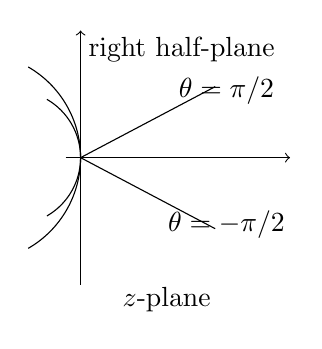
\begin{tikzpicture}[scale=0.95]
\draw[->] (-0.2,0) -- (2.8,0);
\draw[->] (0,-1.7) -- (0,1.7);
\draw (0,-1.45) -- (0,1.45);
\draw (0,0) -- (2.1,0);
\draw (0,0) -- (1.8,0.95);
\draw (0,0) -- (1.8,-0.95);
\draw (0,0) arc (0:60:0.9);
\draw (0,0) arc (0:-60:0.9);
\draw (0,0) arc (0:60:1.4);
\draw (0,0) arc (0:-60:1.4);
\node at (1.35,1.45) {right half-plane};
\node at (1.15,-1.9) {$z$-plane};
\node at (1.95,0.90) {$\theta=\pi/2$};
\node at (1.95,-0.90) {$\theta=-\pi/2$};
\end{tikzpicture}
\hspace{0.8cm}
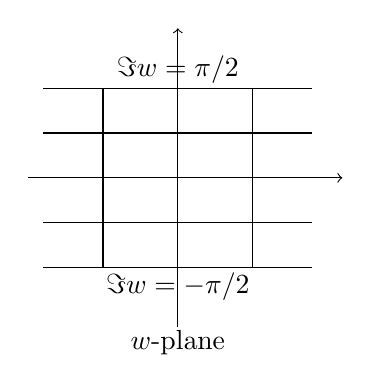
\begin{tikzpicture}[scale=0.95]
\draw[->] (-2.0,0) -- (2.2,0);
\draw[->] (0,-2.0) -- (0,2.0);
\draw (-1.8,1.2) -- (1.8,1.2);
\draw (-1.8,-1.2) -- (1.8,-1.2);
\draw (-1.0,-1.2) -- (-1.0,1.2);
\draw (0,-1.2) -- (0,1.2);
\draw (1.0,-1.2) -- (1.0,1.2);
\draw (-1.8,0.6) -- (1.8,0.6);
\draw (-1.8,0) -- (1.8,0);
\draw (-1.8,-0.6) -- (1.8,-0.6);
\node at (0,1.45) {$\Im w=\pi/2$};
\node at (0,-1.45) {$\Im w=-\pi/2$};
\node at (0,-2.2) {$w$-plane};
\end{tikzpicture}
\caption{The logarithm map sends the right half-plane to a strip.}
\end{figure}

This is the moment when the global geometry begins to touch string theory directly. The strip is exactly the kind of parameter space used to describe an open-string worldsheet. If instead we map the whole plane, then the imaginary direction is periodic modulo \(2\pi\). The strip wraps around and becomes an infinite cylinder. That is the corresponding closed-string picture.

The lecture then turns to another map of the same half-plane, now into the unit disk. The spoken algebra is a little loose, but the endpoint checks strongly support the standard representative
\begin{equation}
w=\frac{z-1}{z+1},
\qquad
z=\frac{1+w}{1-w}.
\end{equation}
This sends \(z=0\) to \(w=-1\), \(z=\infty\) to \(w=1\), and the imaginary axis to \(|w|=1\). So the right half-plane goes to the unit disk.

\begin{figure}[h]
\centering
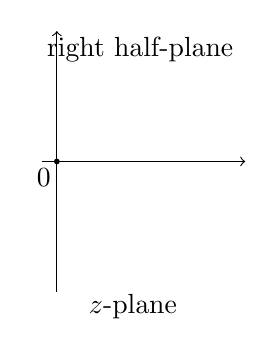
\begin{tikzpicture}[scale=0.92]
\draw[->] (-0.2,0) -- (2.6,0);
\draw[->] (0,-1.8) -- (0,1.8);
\draw (0,-1.6) -- (0,1.6);
\node at (1.15,1.55) {right half-plane};
\node at (1.05,-2.0) {$z$-plane};
\fill (0,0) circle (0.04);
\node at (-0.18,-0.22) {$0$};
\end{tikzpicture}
\hspace{0.9cm}
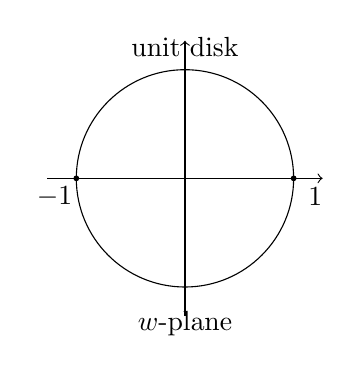
\begin{tikzpicture}[scale=0.92]
\draw[->] (-1.9,0) -- (1.9,0);
\draw[->] (0,-1.9) -- (0,1.9);
\draw (0,0) circle (1.5);
\fill (-1.5,0) circle (0.04);
\fill (1.5,0) circle (0.04);
\node at (-1.8,-0.25) {$-1$};
\node at (1.8,-0.25) {$1$};
\node at (0,1.82) {unit disk};
\node at (0,-2.0) {$w$-plane};
\end{tikzpicture}
\caption{A linear fractional map sends the right half-plane to the unit disk.}
\end{figure}

Susskind emphasizes one more geometric fact here. Under linear fractional, or M\"obius, transformations, circles and lines go to circles and lines. That is why the radial lines and circles of the half-plane picture reappear as arcs and circles in the disk picture. Another form, same physics.

\section{Return To String Theory: The Worldsheet Action And The Disk Picture}

After the break the lecture deliberately changes register. We have set up a good deal of mathematics; now let us see what it is for. Susskind goes back to the earlier \(2\to2\) open-string scattering picture, the strip-like worldsheet he jokingly calls the sports band-aid or butterfly bandage. Time runs from left to right. Two strings come in, join to form one string for a while, and then split back into two strings. The amount of time they spend joined is not fixed; one integrates over it, just as one sums over all histories in quantum mechanics.

The first clarification is about the degrees of freedom. The coordinates \(\sigma\) and \(\tau\) on the worldsheet are merely labels, just as \(x\) and \(y\) were labels on the two-dimensional surfaces earlier in the lecture. The dynamical variables are the spacetime coordinates of points on the worldsheet,
\begin{equation}
X^\mu(\sigma,\tau).
\end{equation}
If we know all the \(X^\mu\), then we know how the worldsheet is embedded in spacetime.

The lecture then reminds us of the Wick rotation. After rotating to Euclidean signature, the weight is of the form \(e^{-S_E}\). The exact chalk marks are partly obscured in the board frame, but the intended quadratic expression is the standard Euclidean worldsheet action,
\begin{equation}
S_E[X]
=
\int d\sigma\,d\tau
\left[
\left(\frac{\partial X^\mu}{\partial \tau}\right)^2
+
\left(\frac{\partial X^\mu}{\partial \sigma}\right)^2
\right].
\end{equation}
Equivalently, the factor in the path integral is
\begin{equation}
\exp\!\left[
-\int d\sigma\,d\tau
\left(
(\partial_\tau X^\mu)^2
+
(\partial_\sigma X^\mu)^2
\right)
\right].
\end{equation}
The square here means a sum over the spacetime index \(\mu\).

Now integrate over all embeddings:
\begin{equation}
\int \mathcal{D}X\,e^{-S_E[X]}.
\end{equation}
This is the path integral over all possible ways the worldsheet can fill spacetime.

\begin{figure}[h]
\centering

\includegraphics[width=0.72\textwidth]{lecture_08_figure_04.png}
\caption{Worldsheet strip sketch with the \(d\sigma\,d\tau\) measure.}
\end{figure}

\begin{figure}[h]
\centering
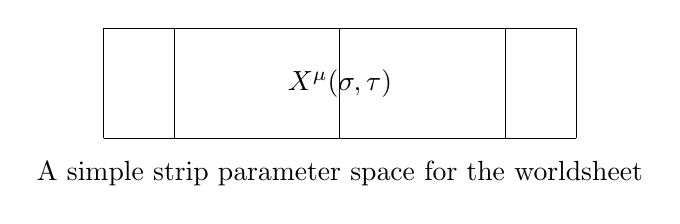
\begin{tikzpicture}[scale=1.0]
\draw (-3,0.7) -- (3,0.7);
\draw (-3,-0.7) -- (3,-0.7);
\draw (-3,-0.7) -- (-3,0.7);
\draw (3,-0.7) -- (3,0.7);
\draw (-2.1,-0.7) -- (-2.1,0.7);
\draw (0,-0.7) -- (0,0.7);
\draw (2.1,-0.7) -- (2.1,0.7);
\node at (0,0) {$X^\mu(\sigma,\tau)$};
\node at (0,-1.15) {A simple strip parameter space for the worldsheet};
\end{tikzpicture}
\caption{A clean redraw of the long narrow strip labelled by the embedding field \(X^\mu(\sigma,\tau)\).}
\end{figure}

At this stage the lecture returns to the geometric freedom earned in the first half. The sports band-aid surface has one boundary. Any one-boundary surface of that sort may be conformally mapped to another one-boundary description, and in particular to a disk. Susskind explicitly says he once worked out the exact map from the sports band-aid to the disk but no longer remembers it. That is fine. We do not need the exact formula. The exact formula is not the point. The point is that the two pictures are conformally equivalent.

\subsection{Question \& Answer}

\paragraph{Question.} How do external momenta enter if the path integral integrates over all \(X^\mu\)?

\paragraph{Answer.} Not through the bulk action alone. This is exactly where Susskind pauses and says that the strip picture is inconvenient. The momentum data are inserted by extra factors associated with the external particles, and the cleanest place to write those factors is the disk picture, where incoming and outgoing strings appear as boundary insertion points.

\section{Vertex Operators, Moduli, And The Electrostatics Reinterpretation}

Once the worldsheet has been redrawn as a disk, the external particles sit at points \(z_i\) on the boundary. For each particle, with spacetime momentum \(k_i^\mu\), we include a factor
\begin{equation}
e^{i k_i\cdot X(z_i)}
=
e^{i k_{i\mu}X^\mu(z_i)}.
\end{equation}
These are the vertex operators. Susskind is careful about their role. They are not the action itself. They are the extra factors that deposit, or inject, momentum into the diagram. They sit inside the path integral, but not inside the area integral that defines the bulk action.

\begin{figure}[h]
\centering

\includegraphics[width=0.72\textwidth]{lecture_08_figure_05.png}
\caption{Euclidean worldsheet weight and vertex insertions.}
\end{figure}

So the open-string tree amplitude has the schematic form
\begin{equation}
\mathcal{A}_n
\sim
\int \mathcal{D}X\,
e^{-S_E[X]}
\prod_{i=1}^n e^{i k_i\cdot X(z_i)}.
\end{equation}
The \(k_i\) are fixed external momenta. The \(X^\mu\) are integrated over, and after that one integrates over the insertion points \(z_i\) on the boundary. Susskind answers this explicitly in the lecture: one does \emph{not} integrate over the momenta. One integrates over the locations where the momenta are inserted.

The same physics can be presented in different coordinate pictures. In the strip picture there is an integration over the relevant separation or time interval. In the disk picture the same freedom appears as integration over the boundary insertion positions. Same picture, same physics, different pictures.

Because of conformal freedom, not all boundary positions are independent. One may use a conformal transformation to place any three boundary points wherever one likes. Therefore the number of remaining integrations is
\begin{equation}
N_{\rm int}=n-3.
\end{equation}
For four open-string external states this leaves a single nontrivial integration.

\begin{figure}[h]
\centering
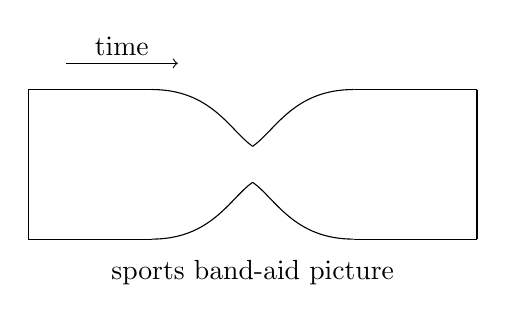
\begin{tikzpicture}[scale=0.95]
\draw (-3,1.0) -- (-1.35,1.0);
\draw (-1.35,1.0) .. controls (-0.55,1.0) and (-0.30,0.45) .. (0,0.24);
\draw (0,0.24) .. controls (0.30,0.45) and (0.55,1.0) .. (1.35,1.0);
\draw (1.35,1.0) -- (3,1.0);

\draw (-3,-1.0) -- (-1.35,-1.0);
\draw (-1.35,-1.0) .. controls (-0.55,-1.0) and (-0.30,-0.45) .. (0,-0.24);
\draw (0,-0.24) .. controls (0.30,-0.45) and (0.55,-1.0) .. (1.35,-1.0);
\draw (1.35,-1.0) -- (3,-1.0);

\draw (-3,-1.0) -- (-3,1.0);
\draw (3,-1.0) -- (3,1.0);
\draw[->] (-2.5,1.35) -- (-1.0,1.35);
\node at (-1.75,1.58) {time};
\node at (0,-1.45) {sports band-aid picture};
\end{tikzpicture}
\hspace{0.9cm}
\begin{tikzpicture}[scale=1.0]
\draw (0,0) circle (1.6);
\fill (1.6,0) circle (0.05);
\fill (0,1.6) circle (0.05);
\fill (-1.6,0) circle (0.05);
\fill (0,-1.6) circle (0.05);
\node at (1.95,0) {$z_1$};
\node at (0,1.95) {$z_2$};
\node at (-1.95,0) {$z_3$};
\node at (0,-1.95) {$z_4$};
\node at (0,-2.45) {disk picture};
\end{tikzpicture}
\caption{One worldsheet, two equivalent descriptions: the strip-like scattering surface and the disk with boundary insertions.}
\end{figure}

Now comes the final unifying move. Because the action is quadratic, the path integrals are Gaussian. In the critical dimension one can do them, and the answer becomes a problem in electrostatics. Each field \(X^\mu\) behaves like an electrostatic potential on the disk. Each component \(k_i^\mu\) of the momentum behaves like a charge inserted at a boundary point. So in the bosonic theory one has \(26\) independent electrostatics problems running in parallel, one for each \(\mu\).

The lecture is slightly garbled at this point, but its intention is very clear. One imagines a disk, places charges on the boundary, solves for the potentials in the interior, computes the electric fields, and from them the electrostatic energies. The distinct \(\mu\)-sectors do not mix; their energies add. After summing those contributions, one exponentiates minus the total energy and integrates over the insertion positions. Schematically,
\begin{equation}
\mathcal{A}_n
\sim
\int d(\hbox{boundary positions})\,e^{-E_{\rm electrostatic}}.
\end{equation}
The lecture does not pause to supply a carefully normalized formula for \(E_{\rm electrostatic}\), and there is no reason to pretend otherwise. What matters is the structural identification: the string amplitude is the exponential of an electrostatic energy, integrated over the worldsheet moduli.

There is one further clarification that the lecture makes explicitly. The \(i\) in the factor \(e^{ik\cdot X}\) is the ordinary imaginary unit. It is not the \(i\) removed by Wick rotation.

\subsection{Question \& Answer}

\paragraph{Question.} If this prescription is so simple, why is the physical theory not finished?

\paragraph{Answer.} Because mathematical elegance is not yet physical realism. In the bosonic theory the path integral gives a sensible finite answer only in the critical dimension \(26\); outside the right dimension one gets infinities. But a \(26\)-dimensional bosonic string theory is plainly not a realistic theory of elementary particles. The extra dimensions must somehow be compactified, and that is where the enormous difficulty begins. Susskind is explicit about this: what has been described here is one simple version of string theory, not the final theory of nature.

He also emphasizes that there are many possible constructions, tied to many possible compactifications. So the lecture ends on a deliberately double note: the formalism is beautiful and rigorous as mathematics, but physically it remains a work in progress. A final late remark fits naturally here as well. The momenta \(k_i\) are not quantized. They are continuous. What becomes quantized is the mass spectrum, built from sums of squares of momentum components.

\section{Summary}

The lecture opens by asking what electrostatics would look like if flux lines could not leave a plane, and it closes by telling us that open-string scattering is, in the end, just such a Laplace problem in disguise. Between those two ends the argument proceeds in a single chain: two-dimensional electrostatics leads to Laplace's equation; Laplace's equation leads to analytic functions; analytic functions are exactly the conformal maps; conformal freedom lets us redraw the worldsheet from strip to disk; and the resulting path integral turns into an electrostatics problem with many kinds of charge.

That is the mathematical core of the chapter. Conformal mapping is not an ornament placed on top of string theory. It is the symmetry that makes the worldsheet description manageable. The final prescription is remarkably simple when it works, and the lecture lets us enjoy that simplicity. But it also ends by narrowing the claim: the bosonic theory lives in the wrong number of dimensions, compactification is hard, and realism is not yet achieved. The mathematics has become clean; the physics is not yet complete.